\subsection{Static Budget-Feasibility Diagnosis (RQ2)}\label{sec:results:c2}

We evaluate the compile-time feasibility diagnosis against frozen confirmatory executions on 350 deep eligible plans under matched budget $B = 8$.

\begin{table}[t]
\centering
\resizebox{0.9\columnwidth}{!}{%
\begin{tabular}{lrr}
\toprule
& \textbf{Obs.: No BE} & \textbf{Obs.: BE} \\
\midrule
Pred. feasible ($\sum a_i \leq B$) & TN = \textbf{76} & FN = \textbf{0} \\
Pred. infeasible ($\sum a_i > B$) & FP = \textbf{128} & TP = \textbf{146} \\
\bottomrule
\end{tabular}}%
\caption{Feasibility confusion matrix on 350 frozen deep plans. Prediction is $\sum a_i > B$ (infeasible); outcome is budget exhaustion (BE). Positive = infeasible, positive outcome = BE.}
\label{tab:confusion}
\end{table}

\noindent Under static allocation, 146 of 350 plans experience budget exhaustion (41.7\%). The feasibility condition $\sum a_i > B$ correctly identifies all 146 as infeasible (recall = 1.0, FN = 0), confirming that budget exhaustion is a necessary consequence of allocation infeasibility under static execution. However, 128 additional plans are predicted infeasible but complete without budget exhaustion (FP = 128), yielding precision = 146 / 274 = 0.533.

The infeasibility condition is \emph{necessary but not sufficient} for budget exhaustion. Plans with $\sum a_i > B$ may still complete if other termination criteria (step limit, LLM-call limit, early convergence) are reached first. Conversely, no plan with $\sum a_i \leq B$ experiences budget exhaustion (TN = 76, FN = 0), confirming that static budget exhaustion under this executor requires allocation infeasibility.

\subsection{Deep-Regime Confirmatory Evaluation (RQ3)}\label{sec:results:deep}

The budget-aware flat planner is evaluated against static allocation on 350 deep eligible plans ($\texttt{structural\_hops} \geq 2$) under matched budget $B = 8$.

\begin{table}[t]
\centering\small
\begin{tabular}{lrrr}
\toprule
& \textbf{Static} & \textbf{Flat} & $\boldsymbol{\Delta}$ \\
\midrule
EM & 0.1714 & \textbf{0.2486} & $+$\textbf{0.0771} \\
BE events & \textbf{146} & \textbf{0} & $-$146 \\
\bottomrule
\end{tabular}
\caption{Confirmatory results on 350 deep eligible plans (matched budget $B = 8$). Flat improves EM by 7.7 points and eliminates all 146 budget-exhaustion events.}
\label{tab:deep}
\end{table}

\noindent \textbf{Answer quality.} The flat planner improves EM by 7.71 points ($+$0.0771, 95\% CI $[+0.049, +0.109]$, exact McNemar $p = 1.4 \times 10^{-6}$, discordant pairs: $b = 30, c = 3$). The effect is statistically significant and practically meaningful on these deep plans.

\noindent \textbf{Budget exhaustion.} The flat planner reduces budget-exhaustion events from 146 to 0 on the same 350 plans, eliminating all static BE under this protocol. This is a direct consequence of the flat planner's allocation constraint $\sum_s a_s \leq B$.

\subsection{Dependency-Sensitive Importance Ablation (RQ4)}\label{sec:results:ablation}

We ablate the chain importance law by comparing the uniform flat planner against a dependency-weighted chain variant on the same 350 deep plans.

\begin{table}[t]
\centering\small
\begin{tabular}{lrrr}
\toprule
& \textbf{Flat} & \textbf{Chain} & $\boldsymbol{\Delta}$ \\
\midrule
EM & 0.2486 & 0.2571 & $+$0.0086 \\
95\% CI & \multicolumn{2}{c}{$[-0.026, +0.043]$} \\
Exact $p$ & \multicolumn{2}{c}{0.7428} \\
\bottomrule
\end{tabular}
\caption{Chain vs.\ flat on 350 deep plans. The chain importance law yields a marginal, statistically insignificant accuracy change (exact McNemar $p = 0.743$).}
\label{tab:ablation}
\end{table}

\noindent The chain variant uses importance $\tau = 2(i+1) - 1$ for slot $i$ in the longest chain, giving downstream slots higher allocation priority. On deep plans, the chain law yields $\Delta$EM $= +0.0086$ ($p = 0.743$, 95\% CI includes zero). The accuracy change is not statistically significant. The final system uses flat for simplicity: the chain-specific importance weighting did not yield detectable accuracy gains over uniform weighting.

\begin{figure}[t]
\centering
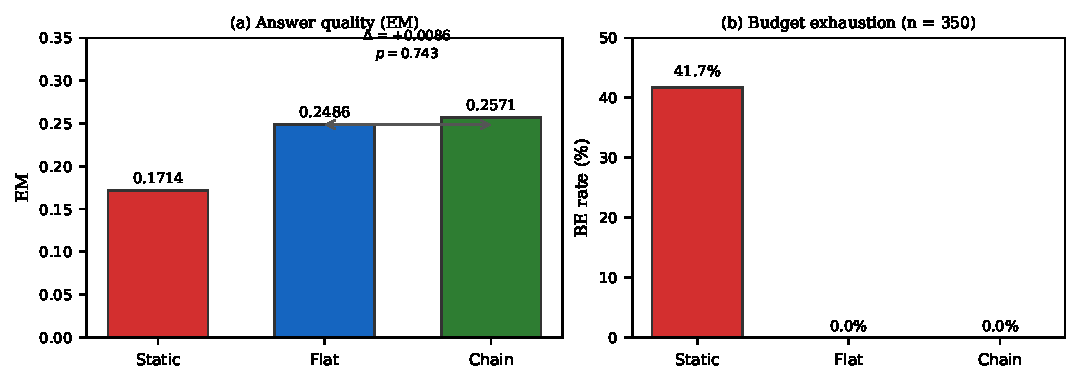
\includegraphics[width=\columnwidth]{figures/three_arm_ablation.pdf}
\caption{Three-arm comparison on 350 deep executable plans (matched budget $B = 8$). (a) Answer quality: chain vs.\ flat $\Delta$EM $= +0.0086$ ($p = 0.743$), not significant. (b) Budget-exhausted rate: flat and chain both eliminate BE; static loses 41.7\% of plans to budget exhaustion. Budget-aware optimization explains the principal improvement; chain importance does not.}
\label{fig:three_arm}
\end{figure}

\subsection{Structure-Gate Exploratory Analysis (RQ5)}\label{sec:results:gate}

\subsubsection{Shallow-regime harm.}
Using the historical three-arm trace (8,632 strict three-arm paired questions under permissive budget), we isolate the shallow stratum ($\texttt{structural\_hops} < 2$, $n = 8{,}085$) and compute the flat vs.\ static treatment effect.

\begin{table}[t]
\centering\small
\begin{tabular}{lrr}
\toprule
& \textbf{Flat $-$ Static} & \textbf{95\% CI} \\
\midrule
EM (exploratory) & $-$\textbf{0.0210} & $[-0.027, -0.015]$ \\
$p$ & \multicolumn{2}{c}{$< 0.001$} \\
\bottomrule
\end{tabular}
\caption{Exploratory shallow-regime flat vs.\ static ($n = 8{,}085$, permissive budget). Flat significantly reduces EM on shallow plans.}
\label{tab:shallow}
\end{table}

\noindent Flat allocation reduces EM by 2.10 points on shallow plans ($p < 0.001$), with the harm concentrated in 2WikiMultiHop ($\Delta$EM $= -0.045$ on hops-0 questions) and near-zero on HotpotQA and MuSiQue shallow strata (secondary analysis, Holm-corrected across dataset $\times$ hops subgroups). This exploratory finding, obtained under the evaluated permissive-budget allocation regime, motivates the gate: applying the budget-aware planner to shallow plans does not help on average and can harm quality.

\begin{figure}[t]
\centering
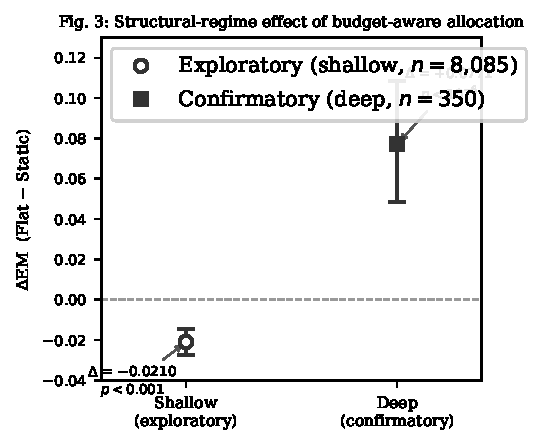
\includegraphics[width=\columnwidth]{figures/regime_effect.pdf}
\caption{Flat $-$ Static $\Delta$EM by structural regime. The shallow effect is \emph{exploratory} (large-scale historical trace, $n = 8{,}085$); the deep effect is \emph{confirmatory} (frozen matched-budget validation, $n = 350$). Independent shallow confirmation was infeasible because the earlier census did not retain full frozen plans for shallow items.}
\label{fig:gate}
\end{figure}

\subsubsection{A' vs.\ always-flat.}
The gated policy A' (flat when $\texttt{hops} \geq 2$ and feasible, static otherwise) is compared against always-flat on the same 8,632 paired trace.

\begin{table}[t]
\centering\small
\begin{tabular}{lrr}
\toprule
& \textbf{A' $-$ Always-Flat} & \textbf{95\% CI} \\
\midrule
EM & $+$\textbf{0.0197} & $[+0.014, +0.026]$ \\
$p$ & \multicolumn{2}{c}{$< 0.001$} \\
\bottomrule
\end{tabular}
\caption{Policy A' vs.\ always-flat (exploratory, $n = 8{,}632$). The gate improves EM by 2.0 points by protecting shallow plans.}
\label{tab:gate}
\end{table}

\noindent The gate improves EM by 1.97 points ($p < 0.001$) by protecting the 93.6\% of questions that are shallow from the flat planner's shallow-regime harm. This is the direct evidence that structure-sensitive dispatch is beneficial.

\subsubsection{Attempted independent confirmation (H-STRUCT-4).}
A confirmatory shallow-regime matched-budget evaluation was pre-registered: n = 1,428 required (power analysis, two-sided $\alpha = 0.05$, 80\% power), drawn from the 6,133 shallow census questions. The V1.2 census, however, did not persist full SlotPlan payloads for shallow questions: only structural metadata and plan hashes were stored, not the SlotPlan JSON required for matched-budget execution. The pre-registered protocol prohibited re-compilation of plans, and no pre-frozen shallow plan snapshots existed in the repository.

The independent shallow confirmation could not be executed. Zero answers were generated, zero models were contacted, and zero counterexamples were produced. The gate's benefit on the shallow regime remains supported only by the exploratory trace; an independent confirmation under the frozen matched-budget protocol remains an open requirement.

\subsection{Population-Level Effect}\label{sec:results:population}

The confirmatory deep stratum constitutes 5.39\% of the validation natural workload (350 / 6,494). The population-level treatment effect of A' is:

$\text{ATE}_{\text{pop}}(\text{A'}) = P(\text{eligible} \wedge \text{executable}) \times \text{ATE}_{\text{exec}} = 0.054 \times 0.0771 = +0.00416 \text{ EM/question}.$

\noindent This is a small but statistically bounded effect (95\% CI $[+0.0025, +0.0059]$, not containing zero). The gate's value is not in large population-level accuracy gains but in eliminating matched-budget budget-exhaustion events on the structural regime where they occur, and in protecting shallow plans from harm.
